% mnras_template.tex
%
% LaTeX template for creating an MNRAS paper
%
% v3.0 released 14 May 2015
% (version numbers match those of mnras.cls)
%
% Copyright (C) Royal Astronomical Society 2015
% Authors:
% Keith T. Smith (Royal Astronomical Society)

% Change log
%
% v3.0 May 2015
%    Renamed to match the new package name
%    Version number matches mnras.cls
%    A few minor tweaks to wording
% v1.0 September 2013
%    Beta testing only - never publicly released
%    First version: a simple (ish) template for creating an MNRAS paper

%%%%%%%%%%%%%%%%%%%%%%%%%%%%%%%%%%%%%%%%%%%%%%%%%%
% Basic setup. Most papers should leave these options alone.
\documentclass[fleqn,usenatbib,letters]{mnras}%added "letters", a4paper is default

% MNRAS is set in Times font. If you don't have this installed (most LaTeX
% installations will be fine) or prefer the old Computer Modern fonts, comment
% out the following line
%\usepackage{newtxtext,newtxmath}
% Depending on your LaTeX fonts installation, you might get better results with one of these:
\usepackage{mathptmx}
%\usepackage{txfonts}

% Use vector fonts, so it zooms properly in on-screen viewing software
% Don't change these lines unless you know what you are doing
\usepackage[T1]{fontenc}
\usepackage{ae,aecompl}


%%%%% AUTHORS - PLACE YOUR OWN PACKAGES HERE %%%%%

% Only include extra packages if you really need them. Common packages are:
\usepackage{graphicx}	% Including figure files
\usepackage{amsmath}	% Advanced maths commands
\usepackage{amssymb}	% Extra maths symbols
\usepackage{cases}  %define a step function

%%%%%%%%%%%%%%%%%%%%%%%%%%%%%%%%%%%%%%%%%%%%%%%%%%

%%%%% AUTHORS - PLACE YOUR OWN COMMANDS HERE %%%%%


%%%%%%%%%%%%%%%%%%%%%%%%%%%%%%%%%%%%%%%%%%%%%%%%%%

%%%%%%%%%%%%%%%%%%% TITLE PAGE %%%%%%%%%%%%%%%%%%%

% Title of the paper, and the short title which is used in the headers.
% Keep the title short and informative.
\title[]{Testing for Flaring Star-Planet Interactions in AU Mic TESS Observations}

% The list of authors, and the short list which is used in the headers.
% If you need two or more lines of authors, add an extra line using \newauthor
\author[E. Ilin et al.]{
E. Ilin$^{1,2}$,\thanks{E-mail: eilin@aip.de}
K. Poppenhaeger$^{1,2}$,
\\
% List of institutions
$^{1}$Leibniz-Institute for Astrophysics Potsdam (AIP), An der Sternwarte 16, 14482 Potsdam, Germany\\
$^{2}$Institute for Physics and Astronomy, University of Potsdam, Karl-Liebknecht-Str. 24/25, 14476 Potsdam, Germany
}

% These dates will be filled out by the publisher
\date{Accepted XXX. Received YYY; in original form ZZZ}

% Enter the current year, for the copyright statements etc.
\pubyear{2020}

% Don't change these lines
\begin{document}
\label{firstpage}
\pagerange{\pageref{firstpage}--\pageref{lastpage}}
\maketitle

% Abstract of the paper
\begin{abstract}
Planets that move in close orbits around magnetically active stars can interact with their magnetic fields in a way that modulates the star's activity. This modulation in phase with the planet's orbit, such as enhanced X-ray activity, chromospheric spots, radio emission, or flares, are the clearest signs of magnetic star-planet interaction (SPI). However, the magnitude of this interaction is difficult to constrain in theory, and the intermittent nature of the interaction is a challenge for observers. 

AU Mic is the most actively flaring star with a recently discovered planet in a 8.6 day orbit, and a promising target for magnetic SPI observations. In this study, we used optical light curves of the young, active M1 star AU Mic obtained by the Transiting Exoplanet Survey Satellite to search for signs of flaring SPI with its innermost companion. 

We found a marginal deviation with orbital phase, and no modulation with the stellar rotation. We suggest that additional 30-120 days of optical monitoring similar to what is provided by TESS would suffice to subtantiate the tentative evidence. If the signal is true, our results can be explained by $\sim8\%$ of the 189 detected flares being triggered by the interaction with the planet. 
\end{abstract}

% Select between one and six entries from the list of approved keywords.
% Don't make up new ones.
\begin{keywords}
stars: individual: AU Mic -- planet-star interactions -- stars: flare -- planets and satellites: individual: AU Mic b
\end{keywords}

%%%%%%%%%%%%%%%%%%%%%%%%%%%%%%%%%%%%%%%%%%%%%%%%%%
%
%-------------------------------------------------------------------

\section{Introduction}

Flares are electromagnetic explosions in the stellar corona that are driven by the dynamics of the surface magnetic fields~\citep{benz2010}. They can be triggered intrisically by the star in isolation, but also by magnetic star-planet interaction (SPI).

In SPI flares, the event is induced by the re-connection of stellar and planetary magnetic field lines~\citep{saur2013,lanza2018,fischer2019}. For this to occur, the planet must revolve around the star in close orbit, so that it moves within the stellar Alfv\'en zone for at least a fraction of its orbit. When the planet is within the Alfv\'en zone, the magnetic field and the energy transported along the field lines as particles or waves can fall back on to the star, whereas outside of it it would be carried away by the stellar wind pressure. 


%When re-connection between star and planet occurs, the energy channelled back into the stellar atmosphere can create an activity hot spot (XXXX Halpha? Xray?) trigger a flare. The footpoint of the connecting field line is expected to move with the planetary orbit (but need not neccessarily be the sub-planetary point).

Several studies of individual systems with close-in and eccentric Hot Jupiters report excess flaring in phase with the planet or close to periastron~\citep{shkolnik2005,pillitteri2011,maggio2015}, but in light of many non-detections of excess flares in similar systems~\citep{figueira2016, fischer2019}, flaring SPI remains an elusive phenomenon. 

One interpretation is that the interaction is so weak and intermittent that the system has to be observed for many orbits of the interacting planet before SPI flares become measurable against the background of intrinsic flares~\citep{shkolnik2008,lanza2009, saur2013,strugarek2015}.

Recently, AU Mic, an M0-M1~\citep{pecaut2013,gaidos2014} pre-main sequence dwarf star has been shown to be a promising candidate for magnetic SPI with its innermost planet~\citep{kavanagh2021}. AU Mic is a member of the $\beta$ Pic young moving group, which is $16-29$ Myr old~\citep{malo2014,binks2014,mamajek2014,bell2015,binks2016,shkolnik2017,miretroig2020}. %Based on its lithium abundance, AU Mic could be a few Myr older than the average group member~\citep{malo2014}. 
%Its rotation period of about $4.862$ d~\citep{plavchan2020, martioli2021} was determined from photometry obtained by the Transiting Exoplanet Survey Satellite~\citep[TESS,][]{ricker2014}.

AU Mic rotates at a $4.862$ d period; it shows strong solar-like differential rotation; possesses a strong, mostly poloidal large-scale magentic field of $>400$ G; and several activity indicators vary in phase with the star's latitude-dependent rotation periods~\citep{klein2021}. Optical light curves obtained by the Transiting Exoplanet Survey Satellite~\citep[TESS,][]{ricker2014} confirm previous observations~\citep{katsova1999, robinson2001, redfield2002} that AU Mic is actively flaring~\citep{martioli2021}.
%Spectral type tends to agree on M1, but effective temperature is lower in Plavchan et al. (2009)

AU Mic b is a Neptune-sized planet ($R_p = 4.3R_{Earth}$) that was first discovered using TESS photometry~\citep{plavchan2020} with an orbital period of $8.463$ d~\citep{plavchan2020,martioli2021}. %A magnetic interaction between star and planet can not only trigger flares, but also enhance X-ray activity and produce chromospheric hot spots~\citep{lanza2009}%, but the exact form and intesity of the interaction is difficult to assess even for individual stars~\citep{strugarek2019} 
\citet{kavanagh2021} predict magnetic SPI with AU Mic b to be observable in the radio regime, a signal indicative of a phenomenon similar to auroral flares observed in the Jupiter-Io system. Since AU Mic is the most actively flaring star among all currently known exoplanet hosts (Ilin et al. in prep.), we may expect SPI flares to also be triggered more readily by AU Mic b. 

In this work, we searched the TESS light curves of AU Mic for signs of flaring SPI. We present our light curve de-trending and flare finding method in Section \ref{sec:detrendfind}, and present the resulting flare catalog in Section \ref{sec:flarecatalog}. In Section \ref{sec:phases}, we show how we can combine flare samples from general time series measurements into a homogeneous data set, and apply this method to test whether flaring SPI signal is present in the TESS observations. We discuss our results and present our conclusions in Sections~\ref{sec:discussion} and \ref{sec:conclusions}.


\section{TESS photometry}
The Transiting Exoplanet Survey Satellite~(TESS,~\citealt{ricker2014}) is an all-sky mission that began operations in 2018, and completed its first full sky scan in April 2020. It is still observing at the time of writing, collecting nearly continuous photometric times series in the 600-1000 nm band for $\sim 27$ d in each observing Sector. About $200\,000$ stars have been observed in 2-min cadence in the first two years of operations with about 20000 targets per Sector. Out of these, from Sector 27 on, 1000 targets were observed at even higher 20-s cadence.

AU Mic was observed in Sector 1 in 2 min cadence and in Sector 27 in 20 s cadence. The light curves reveal strong rotational variability from starspots, vigorous flaring and show transits of two planets, AU Mic b~\citep{plavchan2020,martioli2021} and AU Mic c~\citep{martioli2021}.
% 20000 per sector does not add up, because of stars observed in multiple sectors, the 20000 and 1000 figures can be found here: https://tess.mit.edu/observations/target-lists/
% extended TESS mission https://heasarc.gsfc.nasa.gov/docs/tess/extended.html

\section{Light curve de-trending and flare finding}
\label{sec:detrendfind}
Stellar light curves are time series of flux measurements that vary due to both astrophysical and instrumental effects. Flares are only one of many phenomena like spot variability, transits, eclipses, bursts and dips that can be detected in the data. Accurate automated flare detection algorithms are still challenging to design~\citep{vida2021}, not least due to this intrinsically heterogeneous morphology of light curves. We applied an iterative three-step algorithm to remove all but the variations caused by flares, and derive a realistic noise estimate (Section~\ref{sec:detrend}), then used a two-step $\sigma$-clipping procedure to mark flare candidates and derive their properties~(Section~\ref{sec:flarefind}), and present the resulting flare catalog in Section~\ref{sec:flarecatalog}.

\subsection{De-trending}
\label{sec:detrend}
The light curves were de-trended in three steps, each of which removed variability on decreasing time scales while preserving the flare signal. Typical flare times range from a few minutes to a few hours, and rarely exceed one day in duration. Most stellar variability occurs on longer time scales, except for ultrafast rotational variability in some stars~(Ilin+2021, submitted). The following method was designed with a broad spectrum of Kepler~\citep{borucki2010} and TESS light curve types in mind. Because AU Mic is extraordinarily active, we mark the adjustments made to accomodate that with comments in parentheses. 

First, we fit and subtract a third order spline function that goes through the start and end of any light curve portion that has no gaps longer than 2 h, and through an averaged flux point every 6 h (30 h for stars that are less variable than AU Mic) inbetween. This step removes long term trends as well as starspot variability on time scales of seveal days. If the light curve portion is shorter than 5 d, this step is skipped. 

Second, we iteratively remove strong periodic signal on time scales between 2 h and 5 d from the light curve. Each iteration first masks outlier points using a padded sigma-clipping procedure. For this step, single outliers above $3.5 \sigma$ are masked as pure outliers, and series of $n>1$ data points above $3.5 \sigma$ are masked as flare candidates or other extended outliers and padded with rounded $\sqrt{n}$ masked points before the outliers to capture slow rise phases, and rounded $2\sqrt{n}$ after the series to capture a potential extended decay phase that flares often display. Then we calculate a Lomb-Scargle periodogram for the light curve, and perform a least-square fit with a cosine function using the dominant frequency in the periodogram as a starting point. The cosine fit is then subtracted from the light curve. We iterate five times or until the dominant peak's signal-to-noise ratio drops below 1. 

As a third step, we again apply the padded outlier clipping, and smooth any remaining variability that is not sinusoidal, first with a 6 h and then with a 3 h window 3rd order Savitzky-Golay~\citep{savitzky1964} filter implemented in \texttt{scipy} as \texttt{signal.savgol\_filter}.

These three steps can sometimes overfit the very edges of the light curve, leaving small exponential drops or rises in the flux that affect the quiescent flux level calculation and/or produce false positive flare detections. If the first or the last data point is a $1\sigma$ outlier in the de-trended light curve, we fit an exponential growth or decay function to these fringes.

Finally we estimate the noise in the de-trended light curve using a rolling standard deviation with a 2 h window after padding outliers in the aforementioned way, but now above $1.5 \sigma$ ($2.5 \sigma$ for light curves with lower activity). We interpolated the masked outliers to arrive at a noise in the flare regions that is informed by the flux uncertainty in an adjacent light curve portion.

The result for the light curve in Sector 1 is shown in Fig.~\ref{fig:illustrate_detrend}. The method was inspired by the iterative approach in~\citet{davenport2016} who searched the entire Kepler catalog for flares. We tested our approach on a variety of synthetic and real light curves in the TESS and Kepler archives, so that it can be applied directly to a larger sample.

\textcolor{red}{We provide an example script that shows how to use this method with Kepler and TESS short cadence light curve with \texttt{AltaiPony}.}

\subsection{Flare finding}
\label{sec:flarefind}
We searched the de-trended light curves for flare candidates. For this, we first find an iterative median, and then apply the threshold method introduced by~\citep{chang2015} that requires three consecutive positive outliers $3 \sigma$ above median for a candidate detection. To these data points we then add subsequent data points until one of them falls below a $2 \sigma$ above median threshold in order not to cut off detectable parts of the flare decay phase. This series of data points is then flagged as a flare candidate. For each flare, the pipeline returns the flare start and end points, duration, amplitude, and equivalent duration ($ED$) with uncertainties. The $ED$ is the integrated flare flux $F_{flare}$ divided by the median quiescent flux $F_0$ of the star, integrated over the flare duration~\citep{gershberg1972}:
\begin{equation}
\label{eq:ED}
ED=\displaystyle \int \mathrm dt\, \frac{F_{flare}(t)}{F_0}.
\end{equation}

We tested our de-trending and flare-finding procedure on a range of both real and synthetic light curves that covers all typically observed variability signal patterns, and that contains flare signatures between ones that barely exceed the detection threshold to the largest flares we typically observe. We confirmed all flare candidates by eye, and manually corrected the flare duration in cases where the flare shape was not well captured by the algorithm by adding or subtracting data points to the detection. 

%Events like agrabrighetenings and fireflies that occur when light is reflected off of a passing particle into the detector can cause false positive detections that sometimes look similar to flares. These can be identified as occurring simultaneously in multiple light curves.

%False positives are called fireflies\footnote{\url{https://archive.stsci.edu/files/live/sites/mast/files/home/missions-and-data/active-missions/tess/_documents/TESS_Instrument_Handbook_v0.1.pdf}}, for instance in Sector 27.

%The pipeline produces many false positive events in light curves that are extracted from targets that heavily saturate the detector. In these, flares and astrophysical outbursts cannot be unambiguously distinguished from what is more likely a form of overdrive in the detectors' signal processing. 
\begin{figure*}
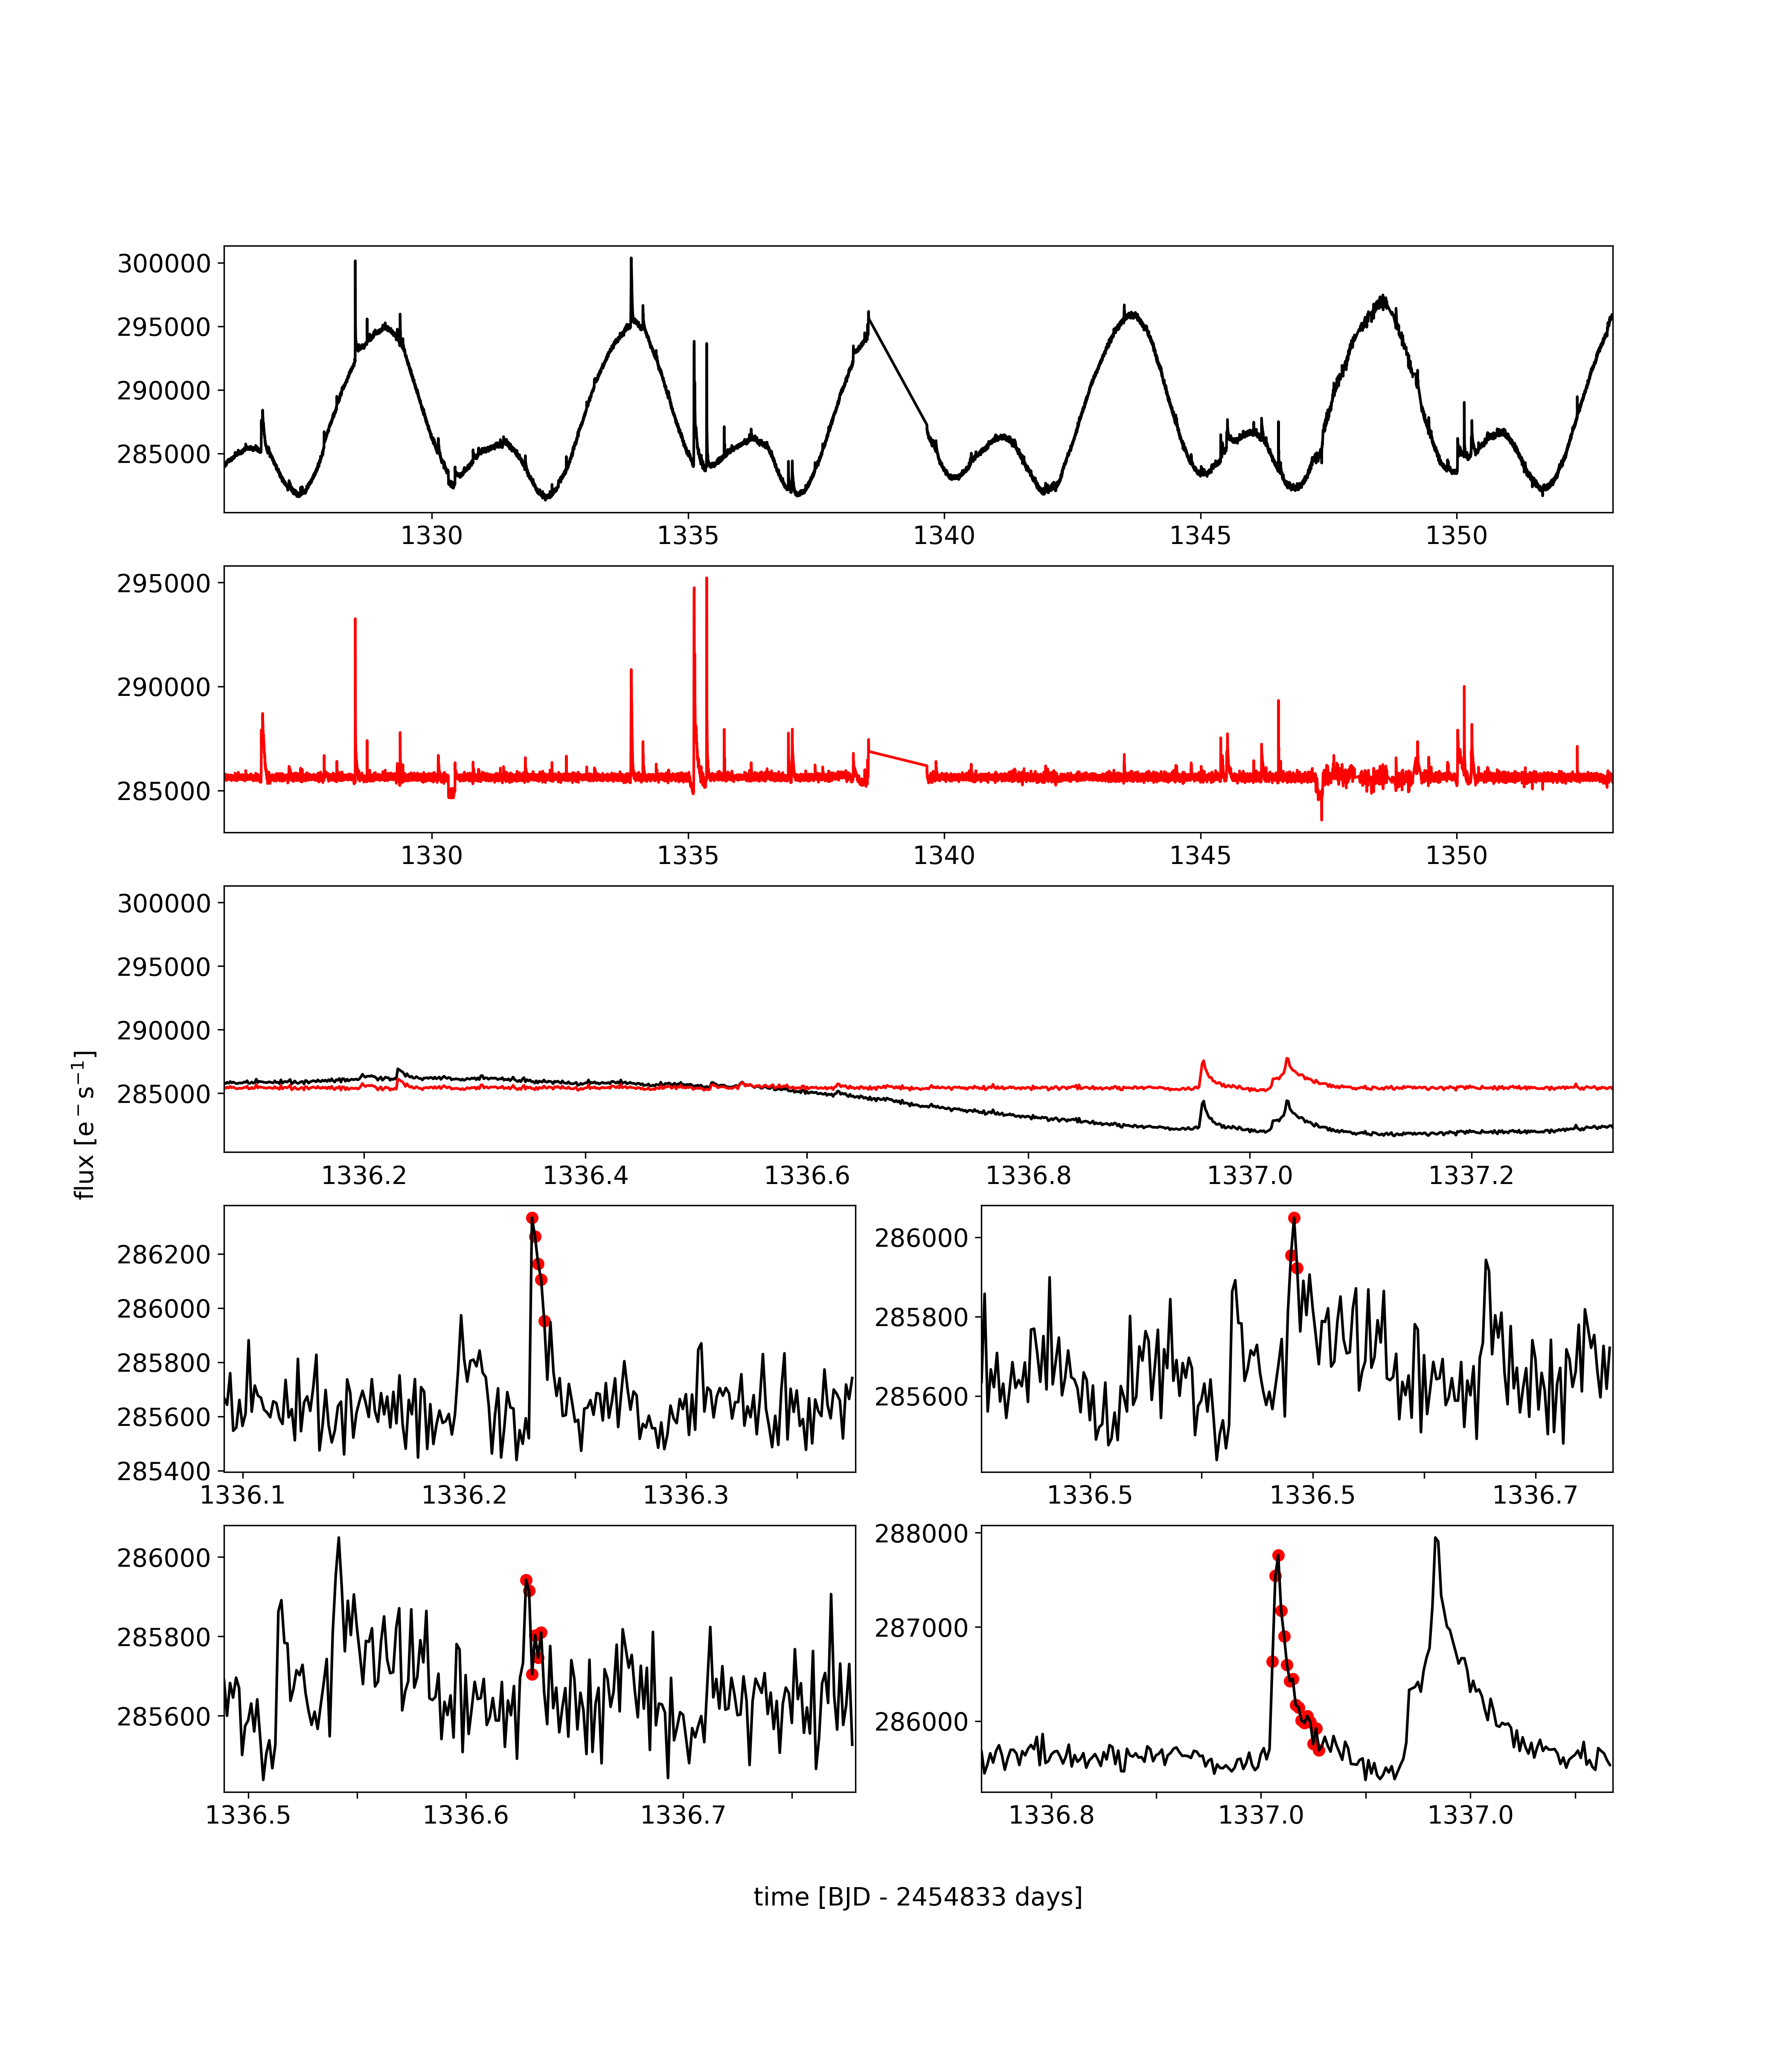
\includegraphics[width=\hsize]{figures/aumic_illustrate_flares.png} 
\caption{Subset of flares detected in the TESS light curve of AU Mic, Sector 1. Top panel: \texttt{PDCSAP\_FLUX} light curve. Second panel from the top: De-trended light curve. Third panel from the top: section from the \texttt{PDCSAP\_FLUX} (black) and de-trended (red) light curve. Four bottom panels: de-trended light curves of flares confirmed in the panel above. The red dots indicate the data points that mark the flares.}
\label{fig:illustrate_detrend}
\end{figure*}

\subsection{Flare catalog}
\label{sec:flarecatalog}
\begin{table}
\caption{Confirmed flare events in the TESS light curves of AU Mic, sorted by orbital phase of AU Mic b. The remainder of the table is available in electronic form.}
\centering
\begin{tabular}{l|ccccc}
\hline
 Sec. &  $t_s$ [BTJD] &  $t_f$ [BTJD] &  orb. phase &    $a$ &         $ED$ [s] \\
\hline
   27 &     2058.2378 &     2058.2526 &       0.001 &  0.007 &  $3.48 \pm 0.04$ \\
   27 &     2058.2584 &     2058.2593 &       0.004 &  0.002 &  $0.10 \pm 0.01$ \\
   27 &     2041.3551 &     2041.3572 &       0.006 &  0.002 &  $0.23 \pm 0.02$ \\
    1 &     1330.4514 &     1330.4709 &       0.007 &  0.003 &  $1.65 \pm 0.03$ \\
   27 &     2041.3690 &     2041.3734 &       0.008 &  0.003 &  $0.70 \pm 0.03$ \\
   27 &     2041.6186 &     2041.6202 &       0.038 &  0.002 &  $0.15 \pm 0.02$ \\
   27 &     2050.1252 &     2050.1259 &       0.043 &  0.003 &  $0.10 \pm 0.01$ \\
   27 &     2050.1724 &     2050.1731 &       0.048 &  0.001 &  $0.07 \pm 0.01$ \\
    1 &     1330.8028 &     1330.8250 &       0.049 &  0.002 &  $1.72 \pm 0.06$ \\
   27 &     2058.7093 &     2058.7148 &       0.057 &  0.004 &  $0.74 \pm 0.03$ \\
\hline

\end{tabular}

\label{tab:flares}
\end{table}

\begin{figure}
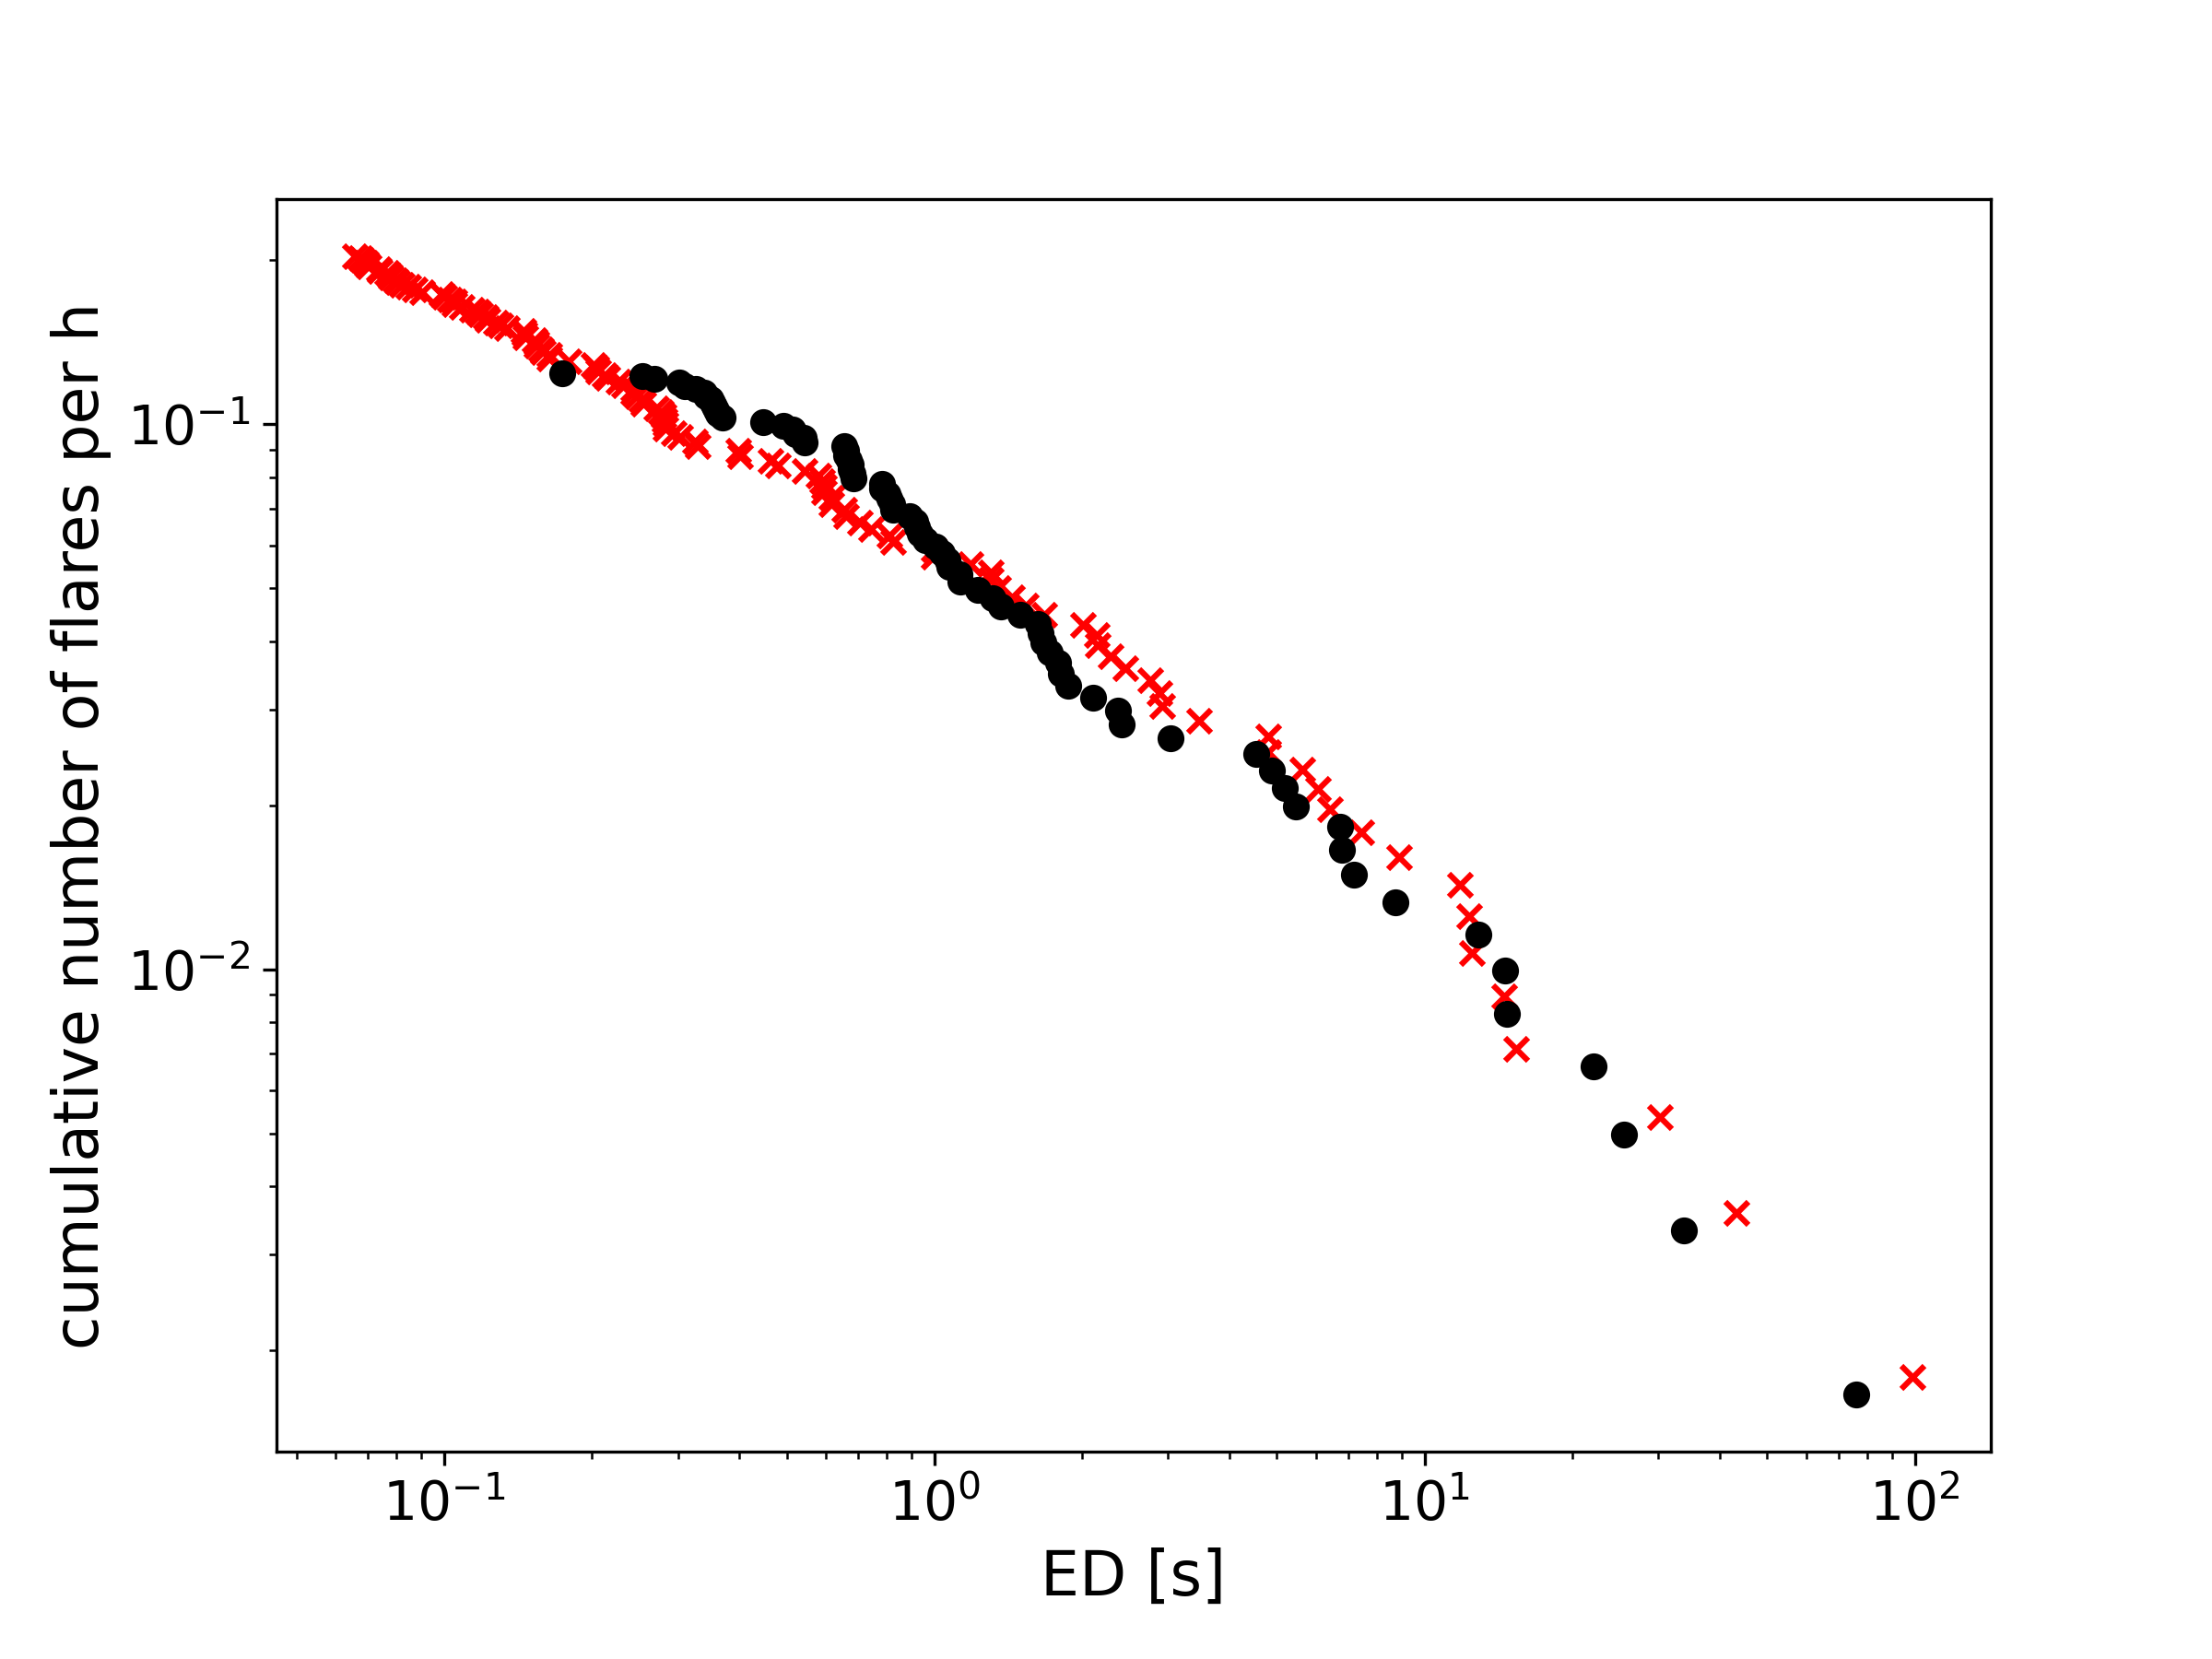
\includegraphics[width=\hsize]{figures/2021_06_11_ffd.png} 
\caption{Flare frequency distributions (FFDs) in $ED$ space obtained from the two TESS light curves of AU Mic.}
\label{fig:ffd}
\end{figure}
We confirmed 75 flares in Sector 1, and 114 flares in Sector 27~(see bottom panels in Fig.~\ref{fig:illustrate_detrend} for examples). We found more flares in Sector 27 because its six times higher observing cadence lowers the detection threshold, which can be seen in the cumulative flare frequency distributions for both Sectors~(Fig.~\ref{fig:ffd}). Overall, we confirmed fewer flares than reported by \citet{martioli2021} who found the 162 and 157 flares in Sector 1 and 27, respectively. We attribute this difference to the respective detection methods. \citet{martioli2021} flagged single $2.5\sigma$ outliers as candidates, while we required three consecutive data points $3\sigma$ above the noise. Table \ref{tab:flares} lists the confirmed flare events with their respective start and finish times $t_s$ and $t_f$, orbital phase of AU Mic b at $t_s$, amplitude $a$ and $ED$.

\section{Flare rate variation with rotational and orbital phases}
\label{sec:phases}

\begin{figure}
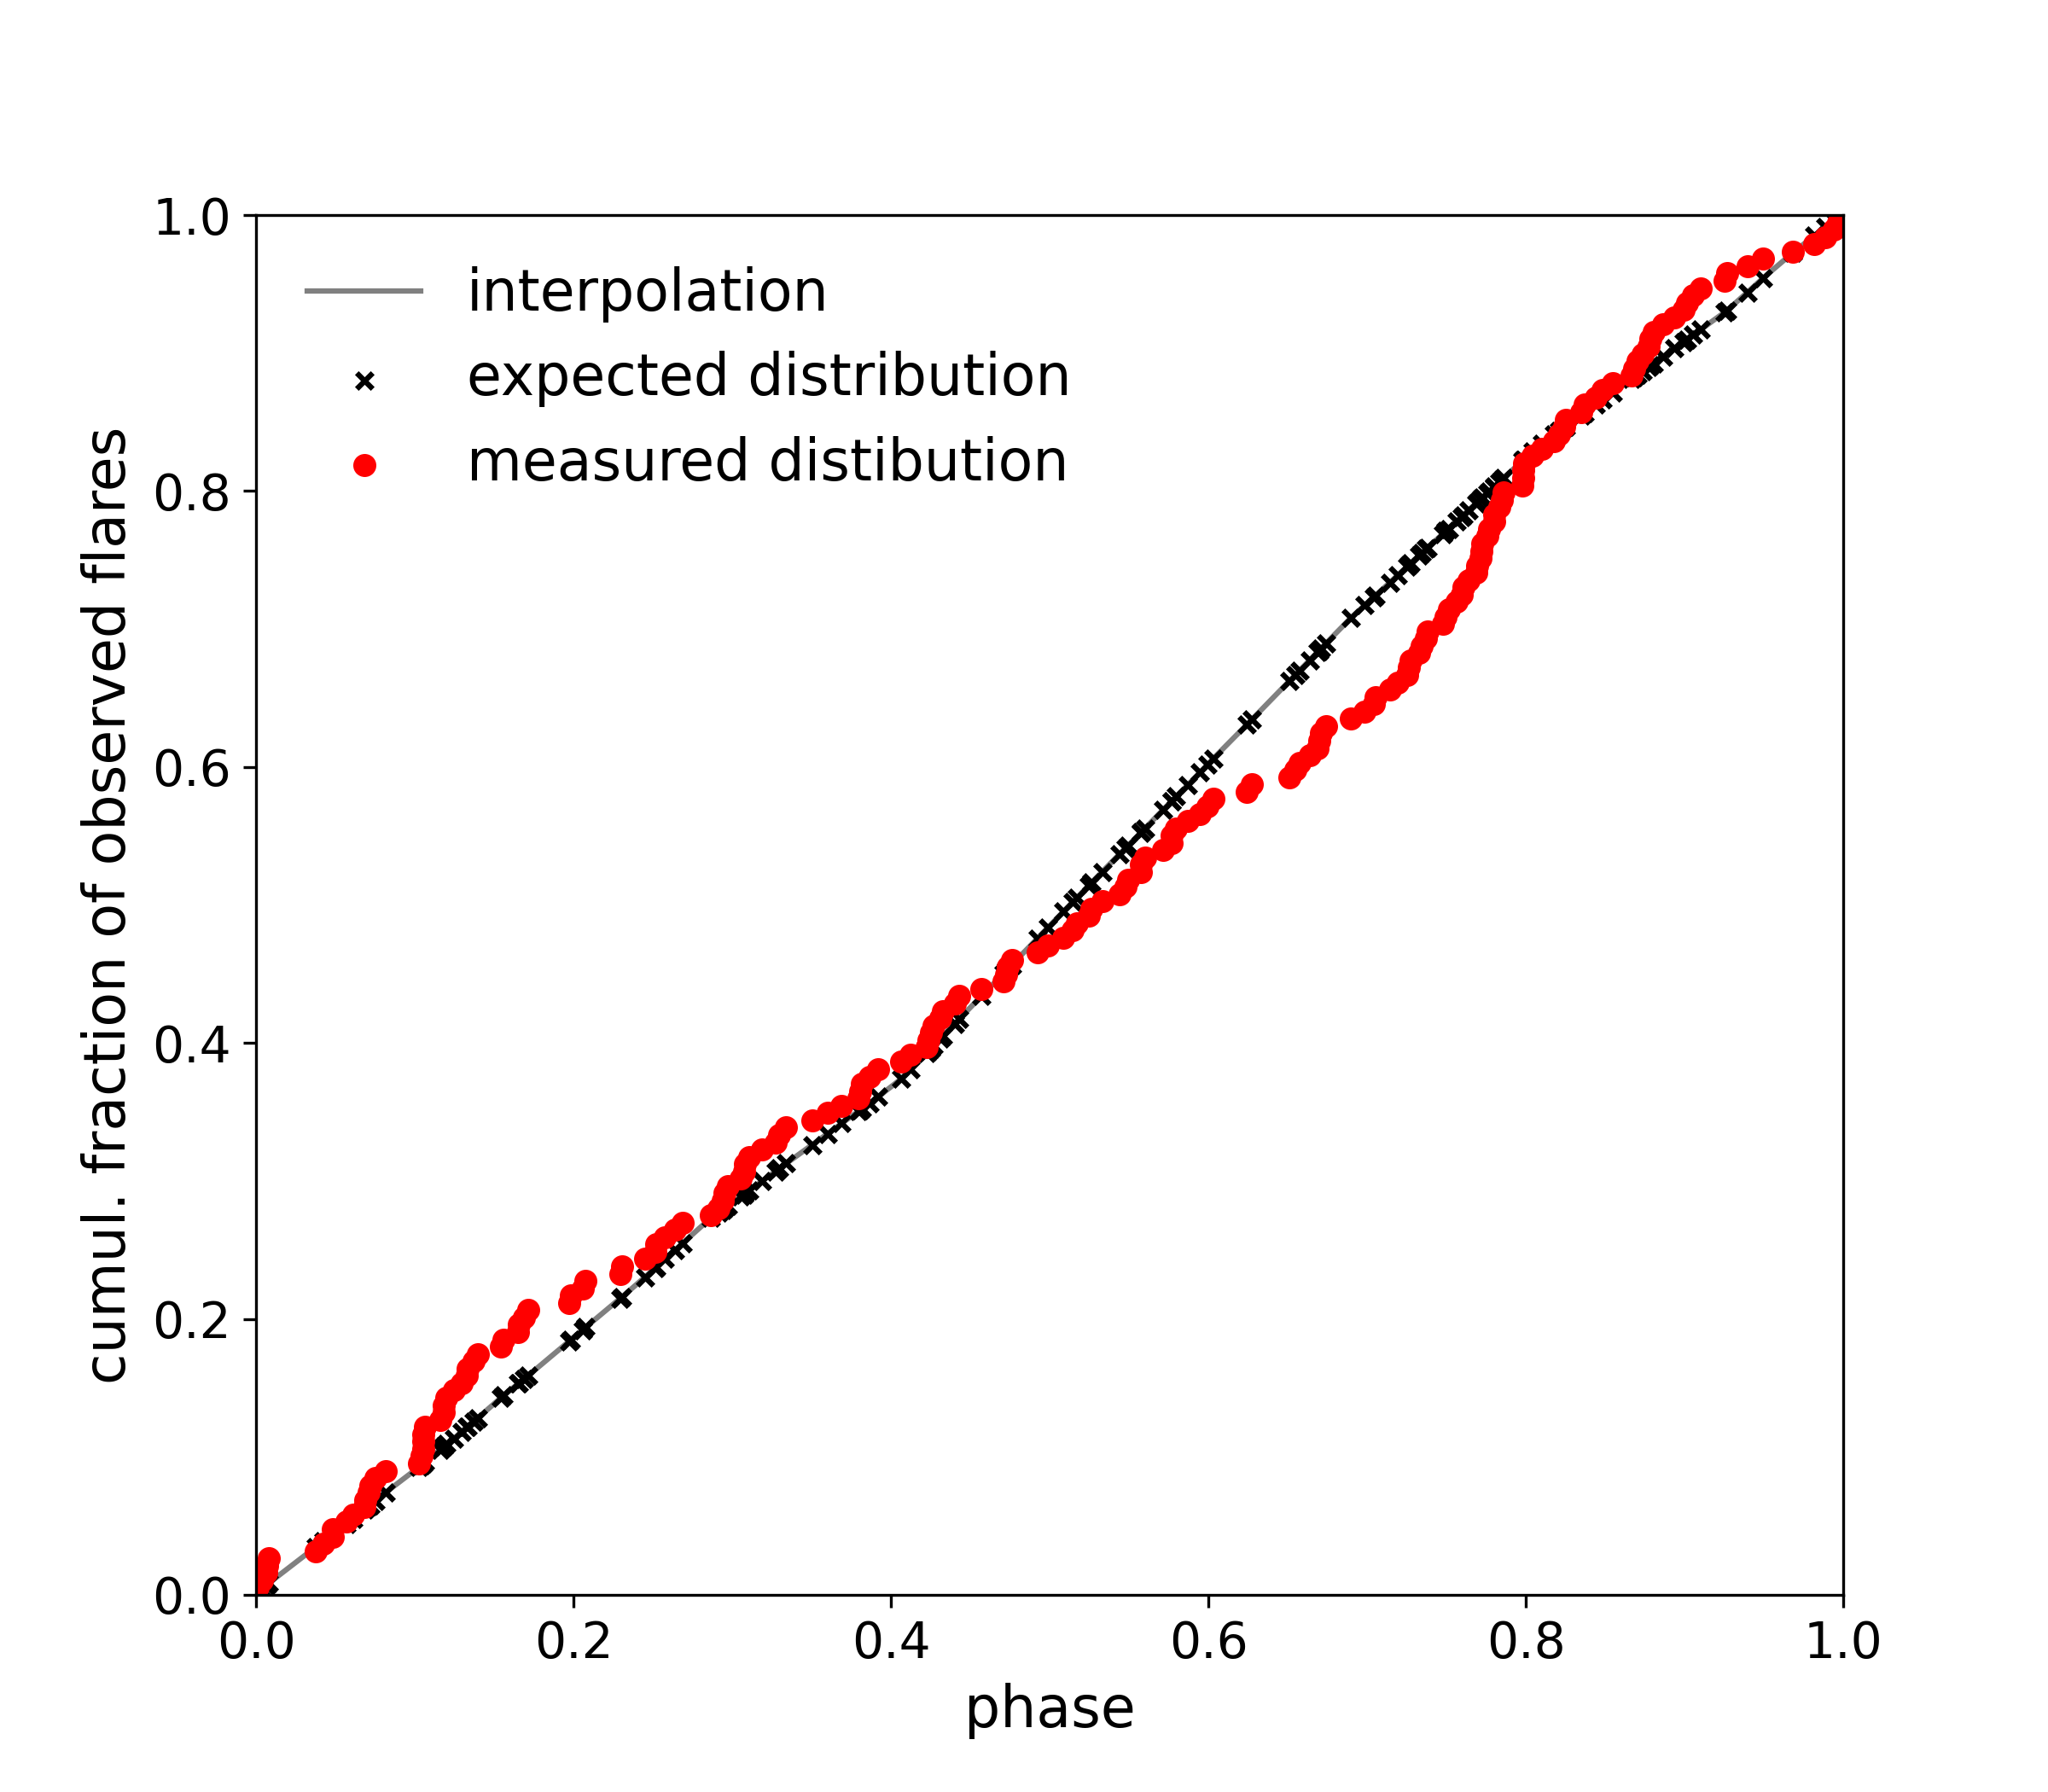
\includegraphics[width=\hsize]{figures/2021_06_08_AUMic_KS_Test_cumdist_total_Both_Sectors_Orbit.png} 
\caption{Cumulative distribution function of flare occurrences as a function of the orbital phase of AU Mic b. Black crosses and black line: The expected distribution with crosses indicating the expected cumulative fraction of observed flares at a given orbital phase. Red circles: Measured cumulative fraction of observed flares as a function of orbital phase. The K-S statistic is defined as the largest absolute vertical distance between the red and the black distribution.}
\label{fig:cumdist}
\end{figure}

\begin{figure*}
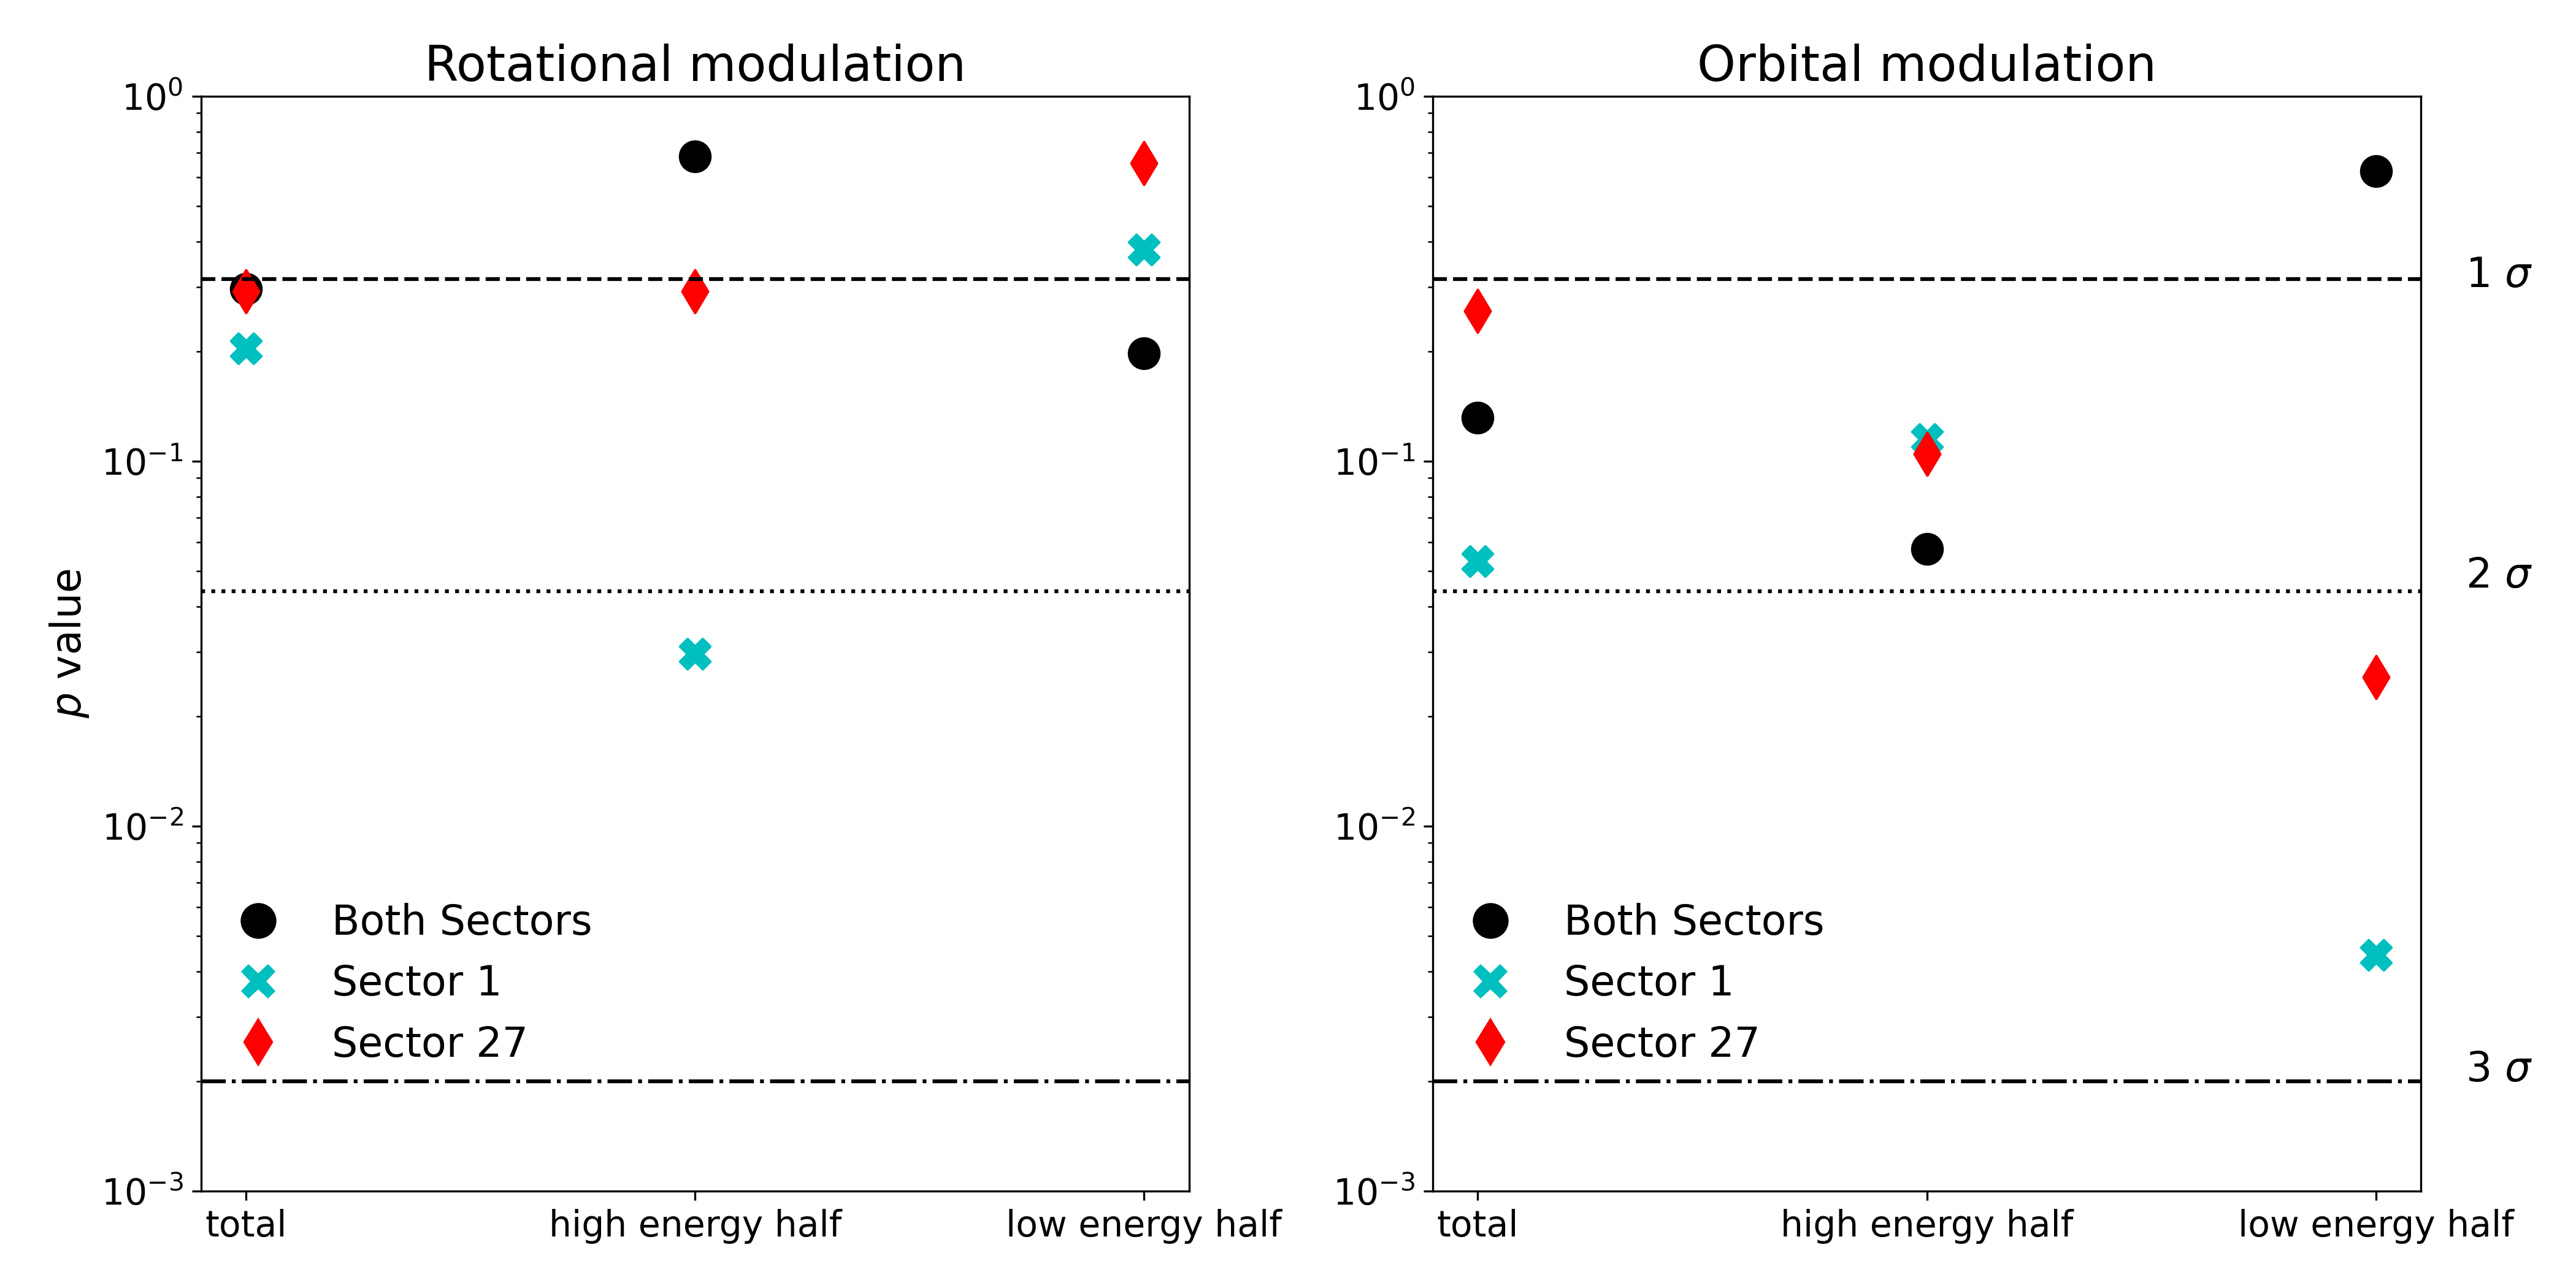
\includegraphics[width=\hsize]{figures/2021_06_09_AUMic_KStests_meta.png} 
\caption{Kolmogorov-Smirnov test results. Black circles, cyan crosses and red diamonds indicate $p$-values obtained using the both available light curve, only the 2-min light curve in Sector 1, or only the 20s light curve in Sector 27, respectively. Each subfigure shows the $p$-values obtained either using the full sample of flares, or 50\% of the most energetic, or 50\% of the least energetic flares, respectively. The $1-,\;2-$ and $3-\sigma$ detection levels are indicated as dashed, dotted and dash-dotted horizontal lines. We found no deviation from a uniform flare distribution at the $3-\sigma$ level with either rotational or orbital phase.}
\label{fig:kstests}
\end{figure*}

\begin{figure}
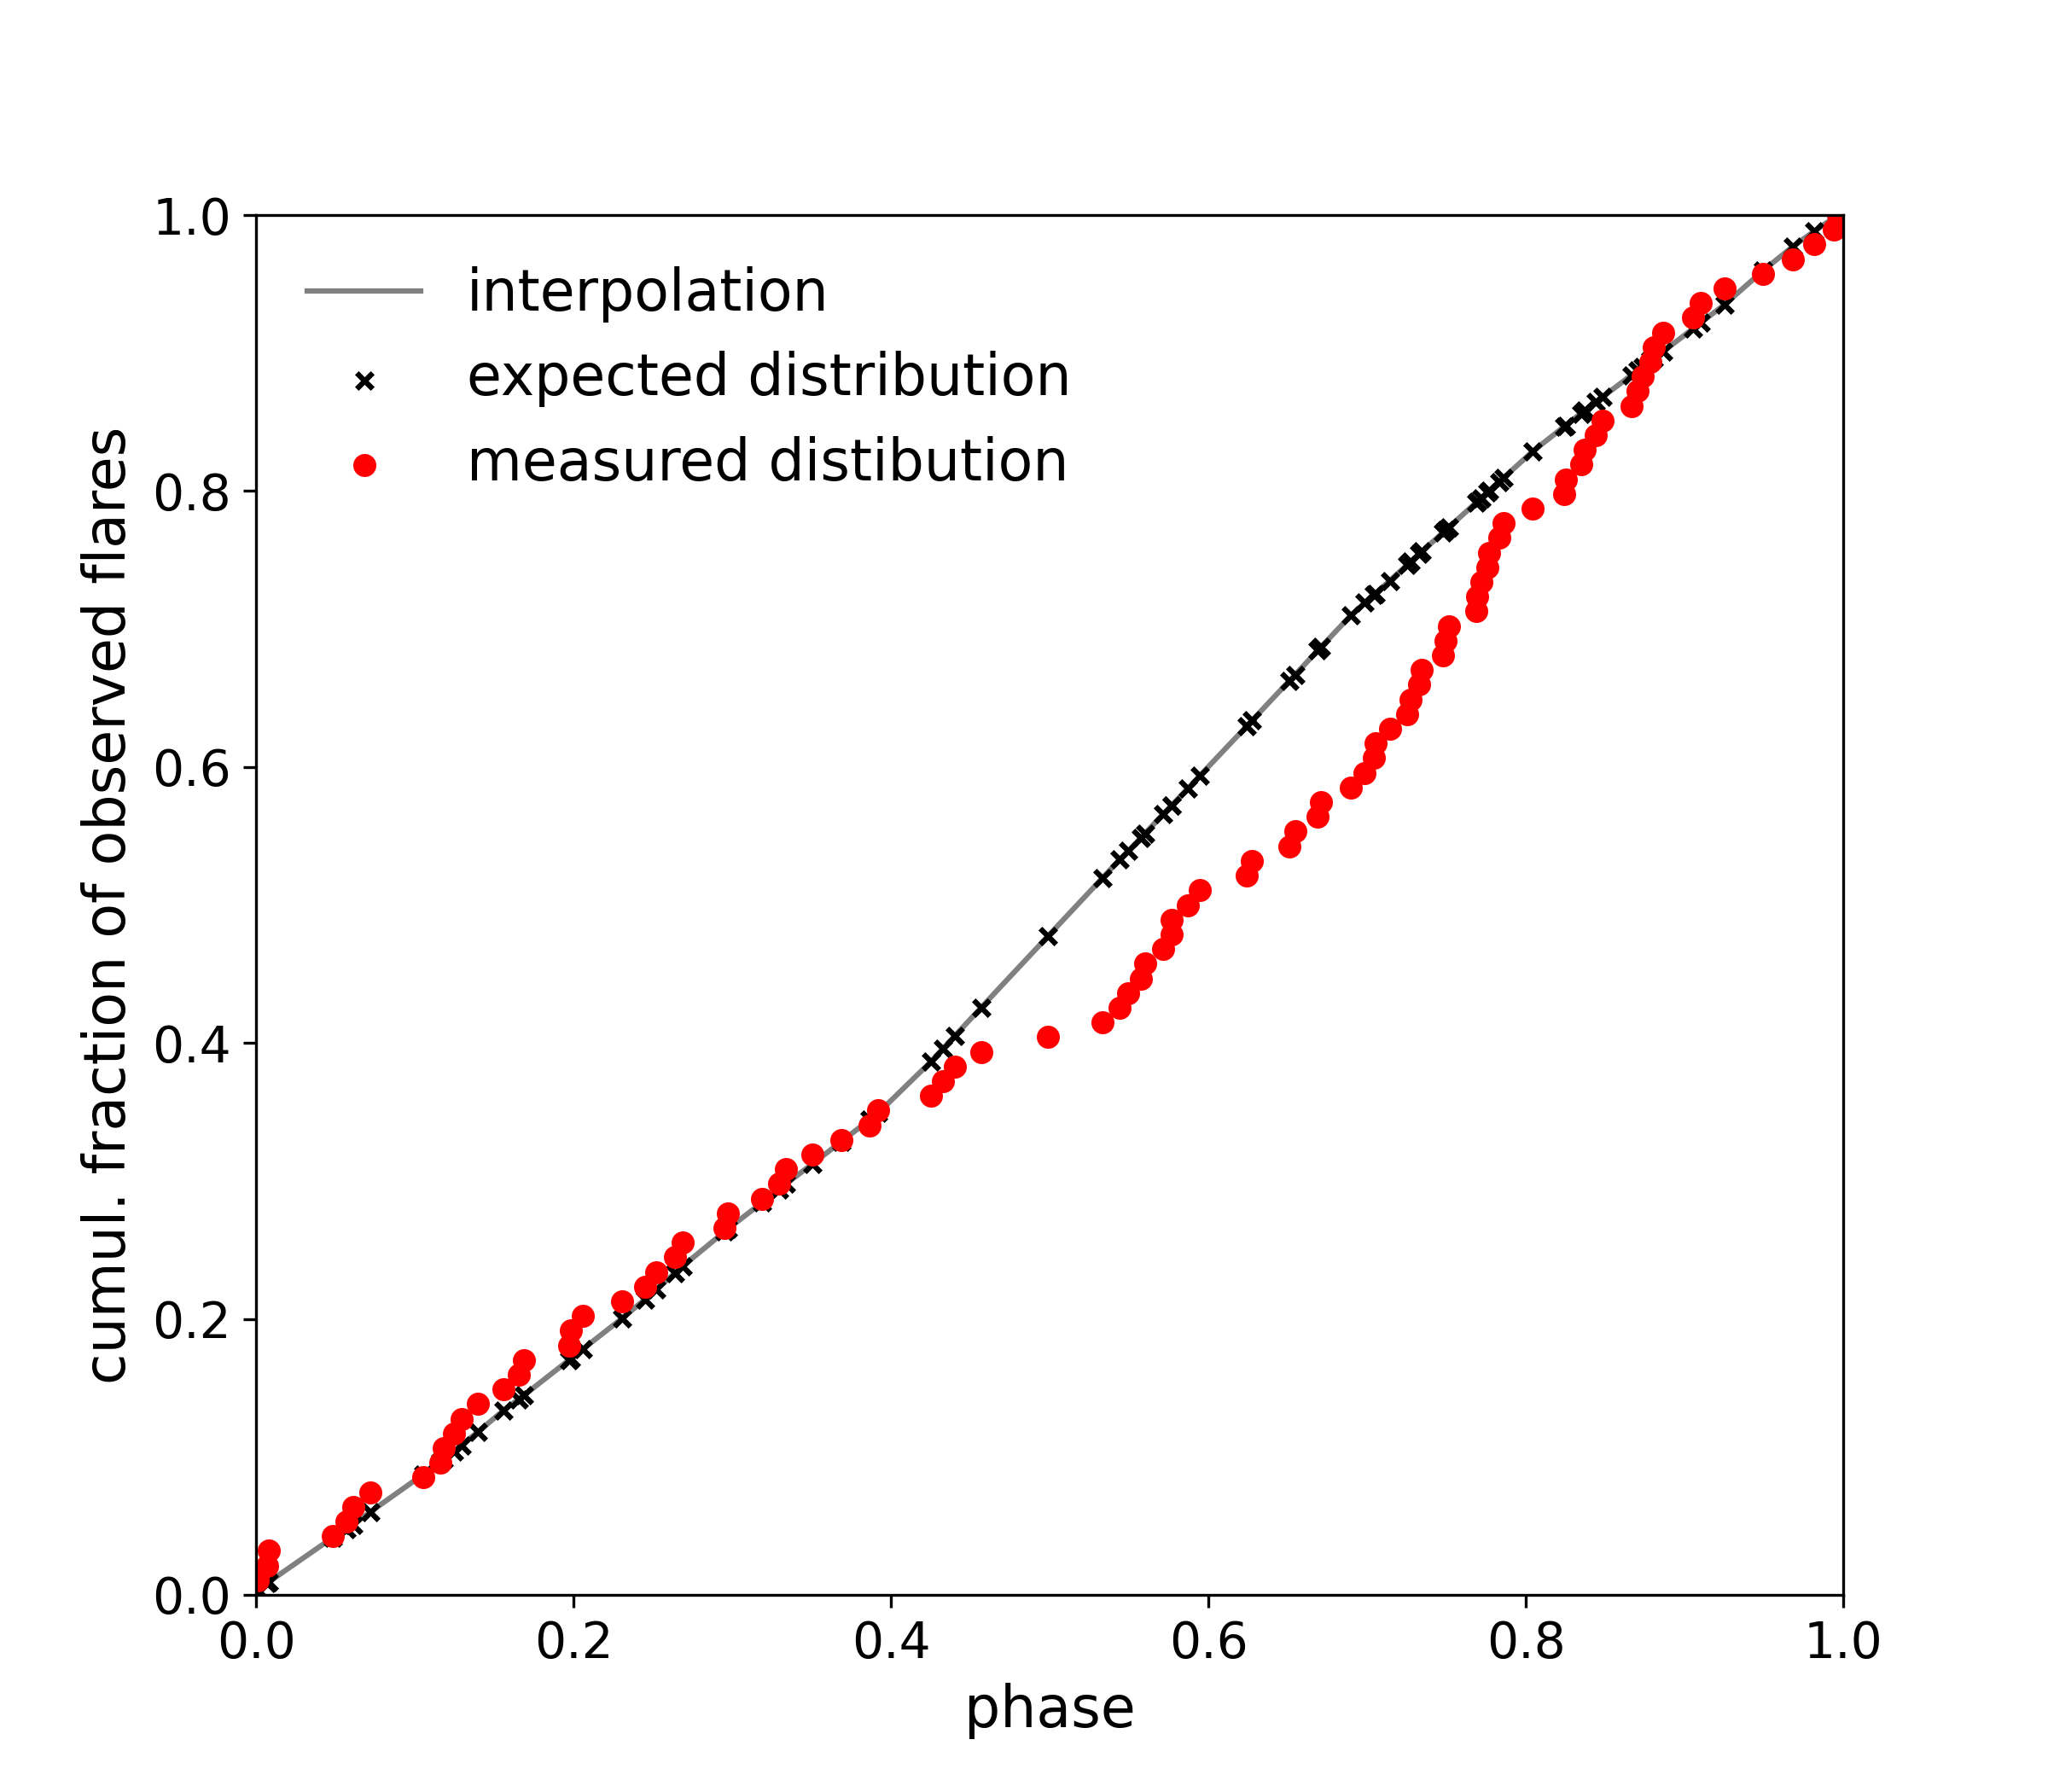
\includegraphics[width=\hsize]{figures/2021_06_09_AUMic_KS_Test_cumdist_high_energy_half_Both_Sectors_Orbit.png} 
\caption{Cumulative distribution function of flare occurrences as a function of the orbital phase of AU Mic b, using the most energetic half of the full flare sample. Colors and symbols are the same as in Fig~\ref{fig:cumdist}}
\label{fig:cumdisthigh}
\end{figure}
\begin{figure}
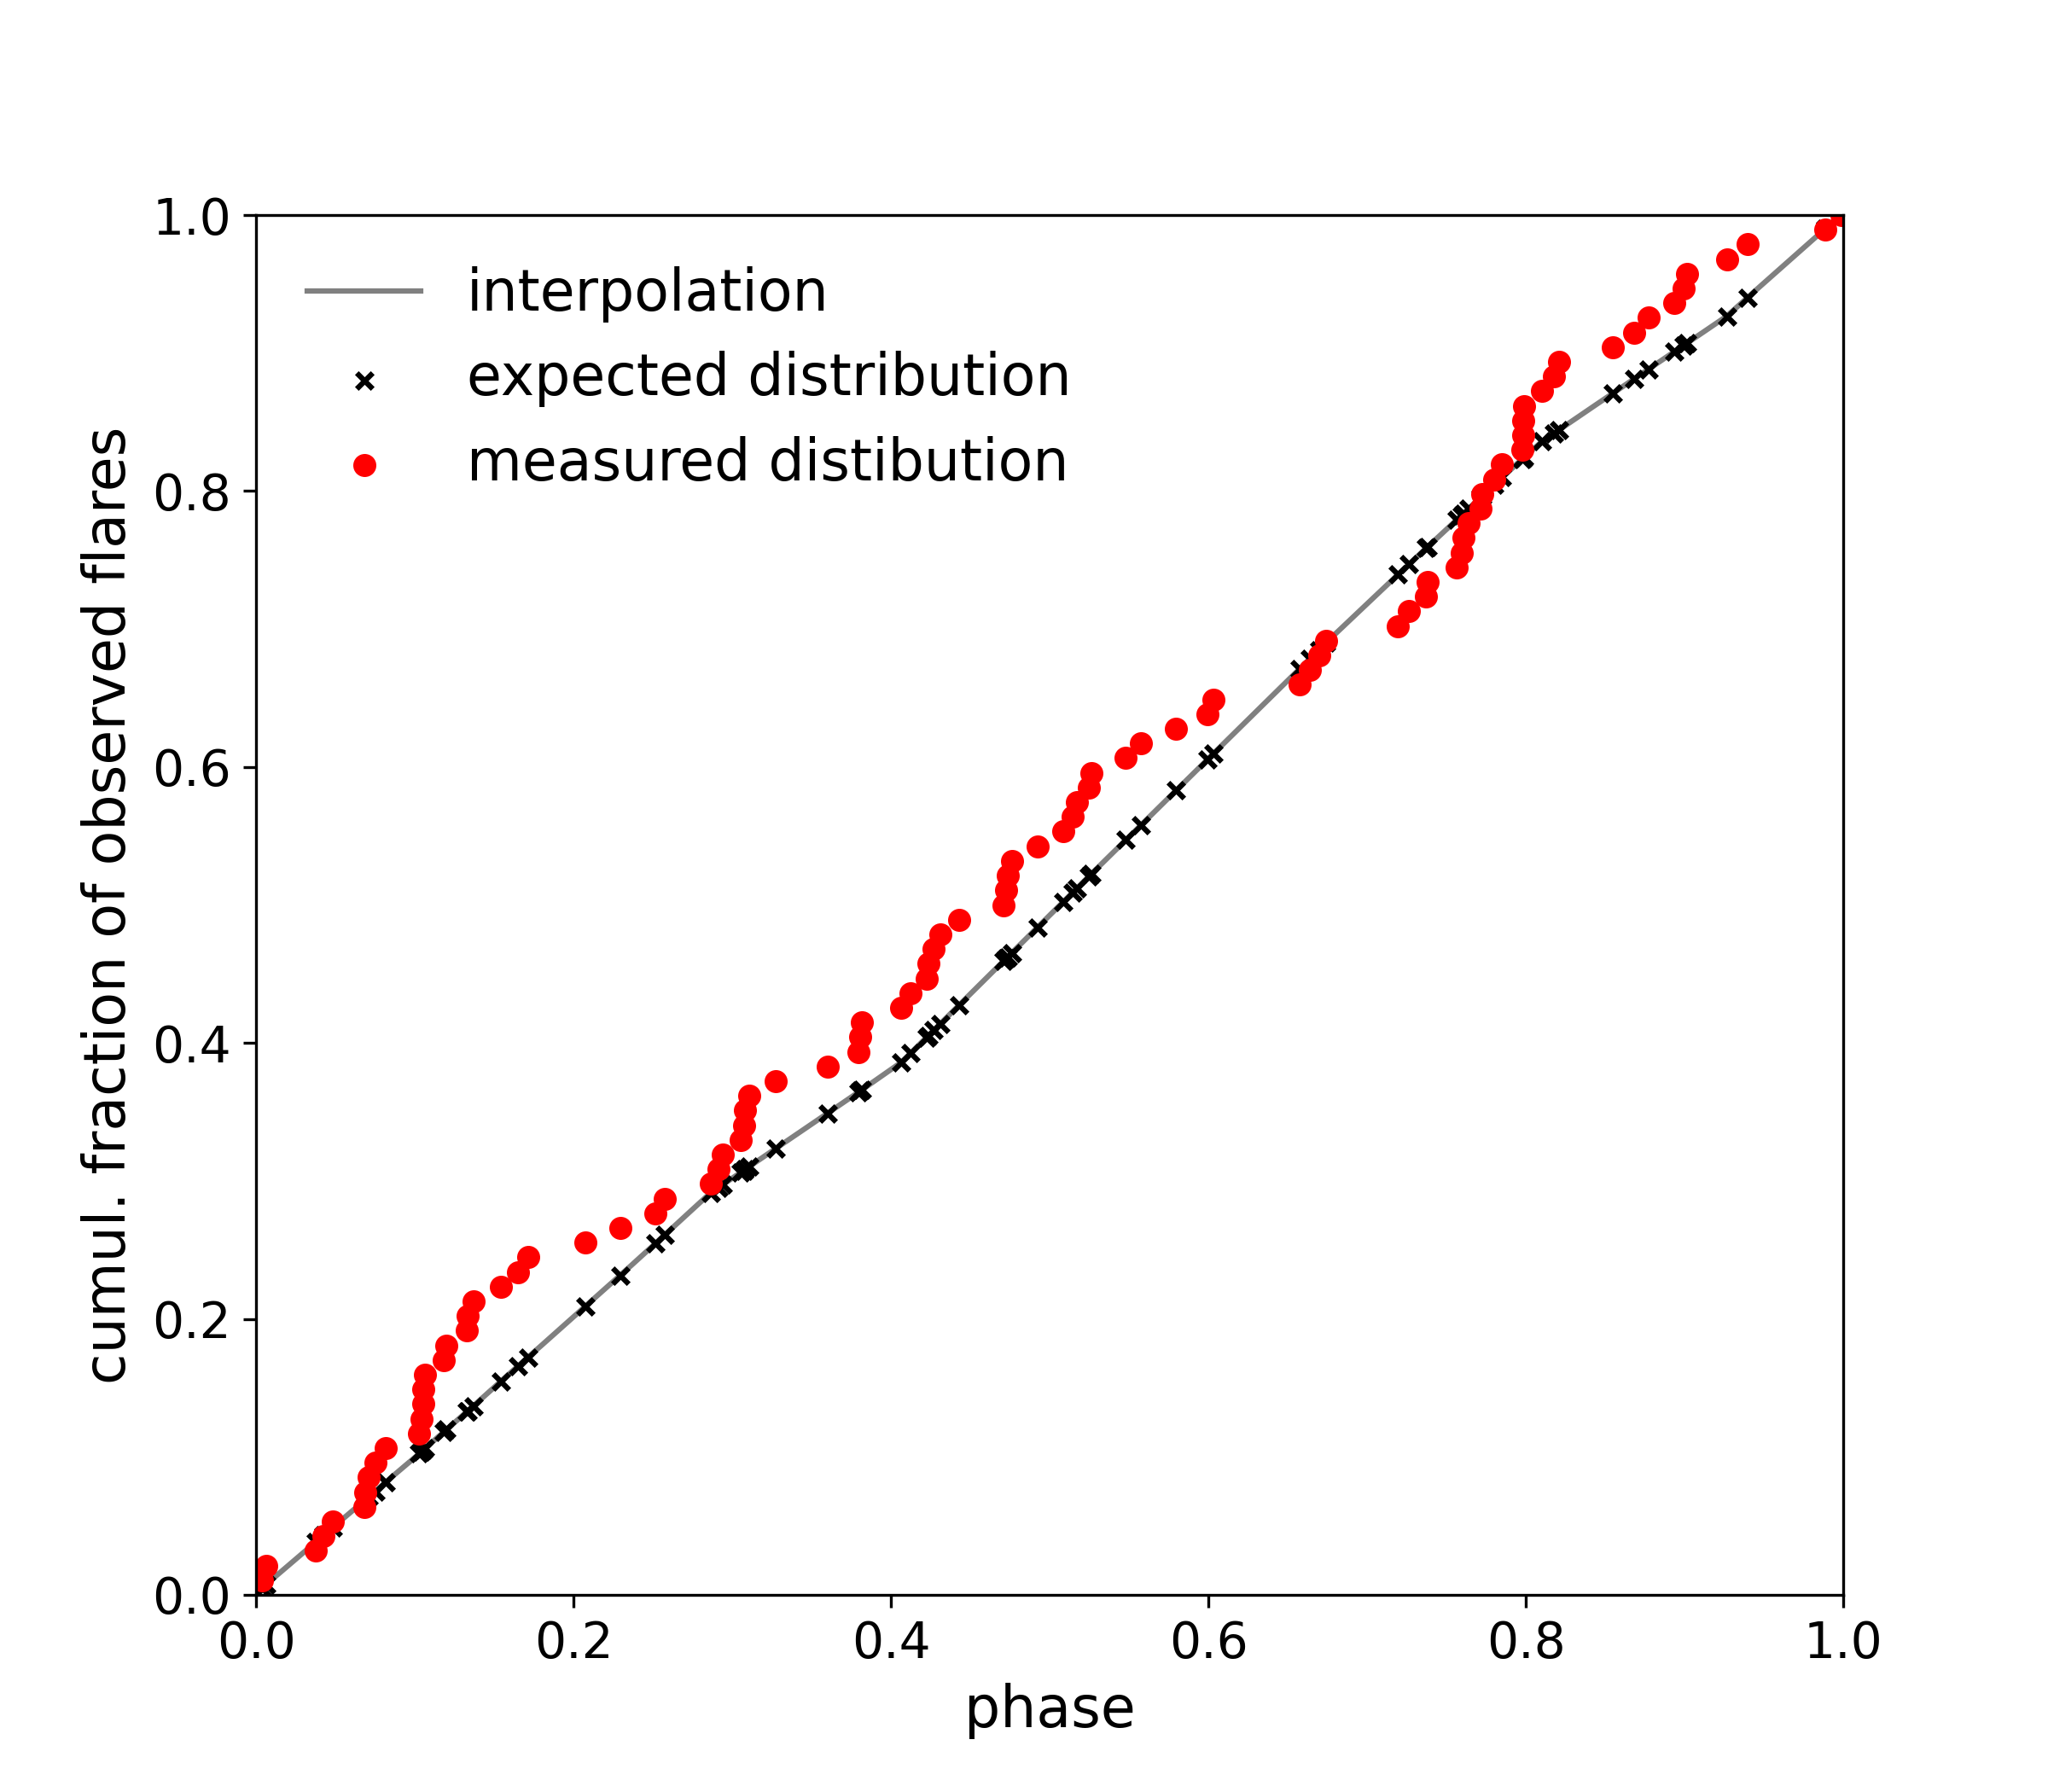
\includegraphics[width=\hsize]{figures/2021_06_09_AUMic_KS_Test_cumdist_low_energy_half_Both_Sectors_Orbit.png} 
\caption{Cumulative distribution function of flare occurrences as a function of the orbital phase of AU Mic b, using the least energetic half of the full flare sample. Colors and symbols are the same as in Fig~\ref{fig:cumdist}}
\label{fig:cumdistlow}
\end{figure}


Stellar flares are thought to occur in the vicinity of active regions on the stellar surface, where magnetic field lines emerge, and magnetic energy can accumulate. AU Mic is a young, extremely active flaring star that is covered with large active regions~\citep{linsky1994, kochukhov2020, plavchan2020}, and possibly a multitude of magnetic loops across the entire corona~\citep{cranmer2013}\textcolor{red}{More on what we know about MF of AU Mic that pertains to its flaring here, and M dwarfs in general}. 

We expect to observe no preference with rotational phase of the star, because flares will randomly occur at the various active regions. If no interaction with the planets in AU Mic's orbit takes place that can trigger flares in certains regions on the star, we also do not expect to observe any dependence of flaring behaviour with orbital phase. We tested this hypothesis by deriving the expected flaring rate distribution under the assumption that no (rotational or orbital) dependence is present, and comparing it against the observed rate. The method works as follows:

We assume that we analyse $N$ light curves $S_k$ with $k\in [1,N]$ that cover observing periods that do not overlap, and each of which has the same flare detection threshold throughout the observing time of the light curve. However, our method allows that the treshold can vary from light curve to light curve, as is the case in our data set for AU Mic.
 
After having searched all $S_k$ for flares, we calculate the deviation from a uniform flare rate distribution with orbital and rotational phase in five steps:
\begin{enumerate}
\item First, we take all $F$ flare occurrence times in AU Mic and derive their orbital or rotational phases $x_i$ with $x \in [1,F]$. 
\item Then, we sort all $x_i$ by phase in ascending order.
\item For each $x_i$, we calculate the number of flares $\hat{n_i}$ we expect to observe in the phase interval $[x_{i-1}, x_i]$, where $x_0\equiv x_F - 1$ (circular boundary condition). Assuming that flare rates are uniformly distributed, we expect to see
$$\hat{n}_i = \displaystyle\sum_{k=1}^N\dfrac{T_{obs, i, k}}{T_{obs, tot, k}} F_k$$
flares, where $T_{obs, tot, k}$ is the total observing time with TESS in each Sector, and the observing time $T_{obs,i,k}$ per phase interval is
$$T_{obs,i,k}=\displaystyle\sum_{x_{i-1}<x<x_i} \Delta t_k,$$
where we sum all observing times $x$ in the phase interval. $\Delta t_k$ denotes the TESS observing cadence (2 min or 20 s). By treating each light curve separately we take into account their different detection thresholds, which allows us to stack flare samples from heterogeneous data. The corresponding measured number of flares in that phase interval is $n_i=1$ per definition.
\item We then calculate the cumulative frequencies of measured and expected flares, $f$ and $\hat{f}$:
$$f(<i) = \dfrac{1}{F}\displaystyle\sum_{j=i}^{i}n_j= \dfrac{i}{F}$$
$$\hat{f}(<i) =  \dfrac{1}{F}\displaystyle\sum_{j=0}^{i}\hat{n}_j = \dfrac{1}{F}\displaystyle\sum_{j=0}^{i}\displaystyle\sum_{k=1}^N\dfrac{T_{obs, j, k}}{T_{obs, tot, k}} F_k$$
\item Finally, we perform a two-tailed one-sample Kolmogorov-Smirnov (K-S) test to check if our observation $f(<i)$ leads us to reject the uniform distribution hypothesis represented by $\hat{f}(<i)$.
\end{enumerate}
We show both $f$ and $\hat{f}$ for the complete sample of orbital flare phases in Fig.~\ref{fig:cumdist}. The expected distribution is not a straight line because the different phase coverages combined with different detection thresholds of the light curves are accounted for in the derivation of the distribution (step (iii)). 

The resulting $p$-values obtained from the K-S test implemented in the \texttt{scipy} method in \texttt{scipy.stats.ks\_1samp} are shown in Fig.~\ref{fig:kstests}. Because AU Mic is seen nearly equator-on, the rotational phase diagrams are consistent with a uniform distribution of flares with stellar longitude (left panel in Fig.~\ref{fig:kstests}), as in the overwhelming majority of M dwarfs~\citep{doyle2018, doyle2019}. 

The observed distribution of flares deviates by $1-2\sigma$ from a uniform distribution of flares with orbital period, which might be attributed to flaring SPI (right panel in Fig.~\ref{fig:kstests}). This effect is stronger in the more energetic half of the flare sample~(Fig.~\ref{fig:cumdisthigh}), but disappears for the least energetic half~(Fig.~\ref{fig:cumdistlow}) when the data from both Sectors are combined. The deviation seen in the cumulative distribution in the full sample also becomes more pronounced in the more energetic subsample~(Fig.~\ref{fig:cumdisthigh}). Interestingly, the effect in the high energy half has a similar magnitude in both Sectors studied separately~(see right panel in Fig.~\ref{fig:kstests}), suggesting that the effect might be persistent over the two year baseline that spans the two TESS Sectors.

Longer monitoring of AU Mic in the optical could clarify whether SPI is present or not. The TESS data comprise $<50$ days of observations, i.e., covering only abbout $5.7$ orbits of AU Mic b. The same magnitude of deviation as observed in the present sample would be significant at the $99\%$ or $99.9\%$ confidence level if the observation baseline could be extended by 62.7 d ($7.4\;P_{orb}$), or 117.3 d ($13.9\;P_{orb}$), respectively. Spot-induced modulation of flare occurrence rates can only be substantiated for spots that are sufficiently long-lived. In contrast, orbital modulation can use combined data from many observational campaigns, even if they are scattered across long periods of time. Moreover, since the spot configuration in AU Mic varies across time~\citep{martioli2021} with spot decay half-life of $110\pm 30$ d~\citep{plavchan2020}, stacking temporally separated observations will eventually average out confounding effects rotational variability. 
\section{Discussion}
\label{sec:discussion}

\begin{table}
\caption{Required observing time in days for a $99\%$ or $99.9\%$ confidence level detection of orbital phase dependent flare rates. Predictions are based on the K-S statistic obtained from the flare rates in Sectors 1, 27, and the combined sample. The required time is shorter for 20 s cadence observations than for 2 min cadence.}
\centering
\input{tables/prediction.tex}
\label{tab:prediction}
\end{table}


\begin{figure*}
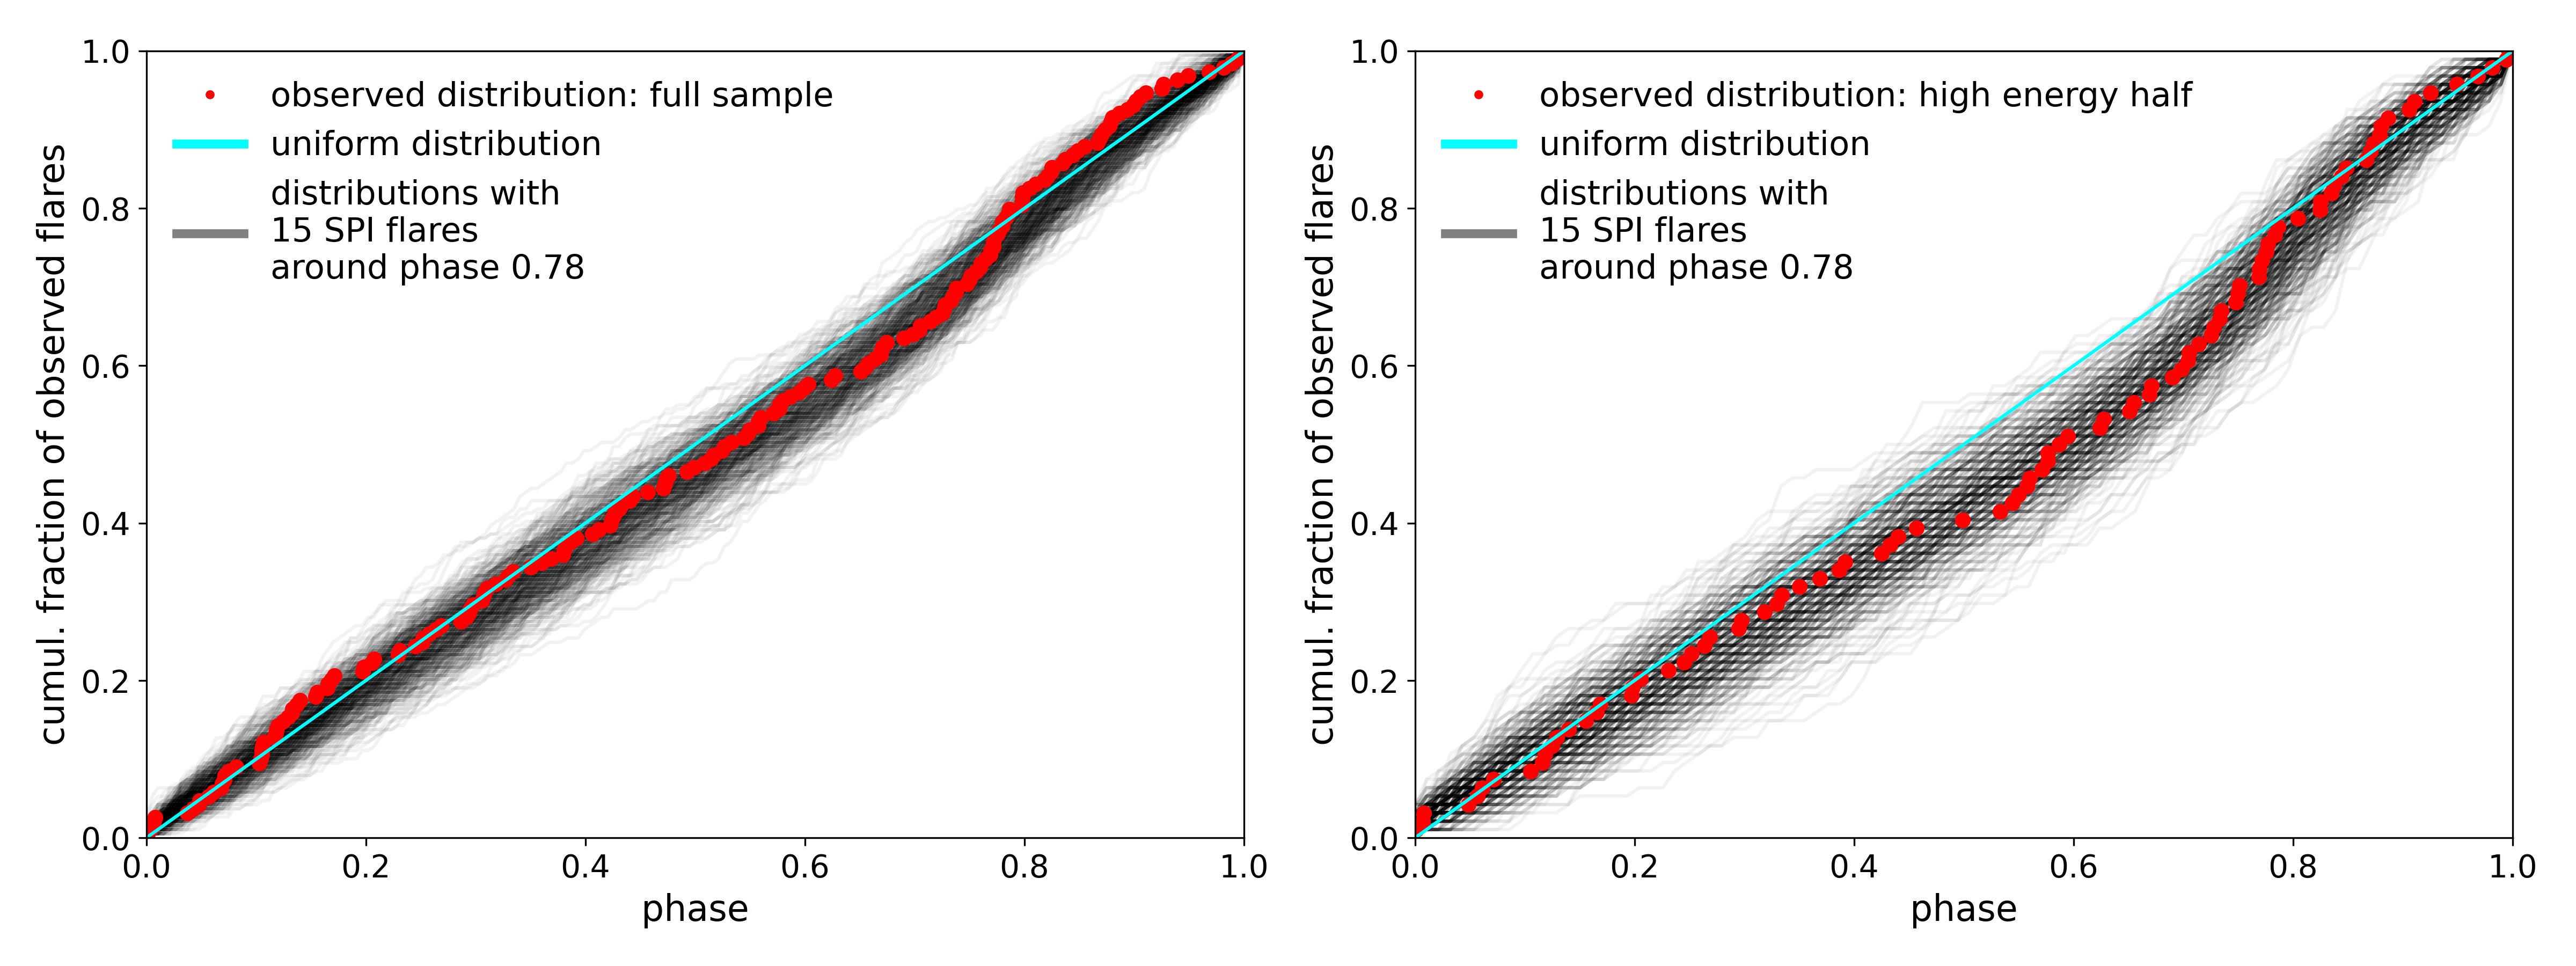
\includegraphics[width=\hsize]{figures/2021_06_10_speculative_SPI_spot.png} 
\caption{Cumulative distributions of flare occurrences as a function of the orbital phase of AU Mic b, compared to synthetic distributions with a flaring SPI component. Red dots in the left and right panel are the same as in Figs. \ref{fig:cumdist} and \ref{fig:cumdisthigh}, respectively. Black lines are instances of distributions, wherein all flares occur at random phases, expect for 15 SPI flares that occur around phase 0.78 in a spot with a $1\sigma$ width of 0.08. The cyan line indicates a completely uniform distribution for comparison. The toy model is consistent with all SPI flares being in the high energy half of the total flare sample.}
\label{fig:speculative}
\end{figure*}



Although the observed distributions of flares do not imply statistically significant SPI signal, if we interpret the marginal detection as sign of SPI, we can ask what causes the departure from a uniform distribution. One possible explanation in line with models is that there is a magnetic spot on the stellar surface whose magentic field lines connect to the planet~\citep{lanza2018, strugarek2019}. Since the star rotates faster than the planet orbits the star, this spot will tend to be ahead of the subplanetary point. 

In the left panel in Fig.~\ref{fig:speculative} we show that our data are consistent with $\sim 15$ out of the 189 observed flares being events in excess of an otherwise uniform distribution with phase. These additional flares are scattered around phase $0.78\pm0.08$, that is, preceding the planet by about a quarter phase, similar to the $60-70^\circ$ predicted by~\citet{lanza2008}. In the right panel in Fig.~\ref{fig:speculative} we reproduce the distribution of the most energetic $50\%$ of the total flare sample, and compare it against the same model as before, but keep the total of 15 SPI flares, which fits the observation. This tentatively suggests that SPI flares are rather energetic, and therefore to be found in the high energy subsample. The relative contribution of SPI flares in this regime ($E_{flare}>XXXX$) is about $\sim16\%$ , whereas it is $\sim8\%$ in the full sample ($E_{flare}>XXXX$). 

Since flaring is a statistical phenomenon, where individual flares are very difficult to predict even on the Sun~\citep{barnes2016}, and SPI flares are also expected to vary orbit to orbit in number and intensity~\citep{shkolnik2008,lanza2009, saur2013,strugarek2015}, it is challenging to identify flares as triggered by SPI as compared to intrinsic flares. Perspectively, a difference in the flare frequency distribution (Fig.~\ref{fig:ffd}) might indicate the presence of SPI, if SPI flares only occurred above an observable energy threshold. The effect could arise as a kink in the power law distribution once a sufficiently large sample of flares accumulates and small differences in the distributions can be disentangled from detection efficiency effects and statistical uncertainty.


\section{Conclusions}
\label{sec:conclusions}
A statistically significant orbital phase dependence of flaring behaviour is the closest we can get to detecting flaring SPI directly. Using high cadence TESS observations of AU Mic, we find weak hints of flaring SPI, and no rotational variability in flare occurrence rates. If the marginal  signal in phase with the orbit of the innermost planet AU Mic b can, however, be interpreted as emerging SPI signal, e.g., from an active spot with a steady phase lag towards the planet, we argue that further monitoring of AU Mic may reveal the interaction. 
Using the method introduced in this work, a longer observing baseline with TESS, covering additional 30--120 days in 2 min cadence, and light curves from other surveys, optical or in other flare-sensitive wavelength bands, can be stacked consistently to confirm or reject the flaring SPI hypothesis for AU Mic. It would also allow us to measure the strength of the interaction, which is difficult to constrain in theory~\citep{strugarek2019}, and discriminate different physical models of flaring SPI~\citep{lanza2018}. We argue further that long gaps on time scales of months to years betweeen consecutive light curves will help average out any confounding rotational variability signal, but should leave the SPI signal fully intact.

In an upcoming study, we will apply the methods of flare finding and orbital phase analysis presented here to a large sample of star-planet systems with known close-in planets to increase the total number of orbits covered, and to probe the effects of orbital distance and star-planet mass ratio on the presence and intensity of flaring SPI.
\section*{Acknowledgements}
EI acknowledges support from the German National Scholarship Foundation. KP acknowledges support from the German Leibniz Community under grant P67/2018. We made use of numpy~\citep{numpy2020} and pandas~\citep{pandas2010,pandas2020software}. This research has made use of the SIMBAD database, operated at CDS, Strasbourg, France~\citep{wenger2000}. This paper includes data collected with the TESS mission, obtained from the MAST data archive at the Space Telescope Science Institute (STScI). Funding for the TESS mission is provided by the NASA Explorer Program. STScI is operated by the Association of Universities for Research in Astronomy, Inc., under NASA contract NAS 5-26555.

\section*{Data Availability}
TESS light curves are publicly available through the Mikulski Archive for Space Telescopes (\url{https://mast.stsci.edu/portal/Mashup/Clients/Mast/Portal.html}).
\textcolor{red}{Where shall we store the full flare table?}
%This publication makes use of data products from the Two Micron All Sky Survey, which is a joint project of the University of Massachusetts and the Infrared Processing and Analysis Center/California Institute of Technology, funded by the National Aeronautics and Space Administration and the National Science Foundation.

%This work has made use of data from the European Space Agency (ESA) mission {\it Gaia} (\url{https://www.cosmos.esa.int/gaia}), processed by the {\it Gaia} Data Processing and Analysis Consortium (DPAC, \url{https://www.cosmos.esa.int/web/gaia/dpac/consortium}). Funding for the DPAC has been provided by national institutions, in particular the institutions participating in the {\it Gaia} Multilateral Agreement.
%%%%%%%%%%%%%%%%%%%%%%%%%%%%%%%%%%%%%%%%%%%%%%%%%%

%%%%%%%%%%%%%%%%%%%% REFERENCES %%%%%%%%%%%%%%%%%%

% The best way to enter references is to use BibTeX:

\bibliographystyle{mnras}
\bibliography{bibliography}


% Alternatively you could enter them by hand, like this:
% This method is tedious and prone to error if you have lots of references
%\begin{thebibliography}{99}
%\bibitem[\protect\citeauthoryear{Author}{2012}]{Author2012}
%Author A.~N., 2013, Journal of Improbable Astronomy, 1, 1
%\bibitem[\protect\citeauthoryear{Others}{2013}]{Others2013}
%Others S., 2012, Journal of Interesting Stuff, 17, 198
%\end{thebibliography}

%%%%%%%%%%%%%%%%%%%%%%%%%%%%%%%%%%%%%%%%%%%%%%%%%%

%%%%%%%%%%%%%%%%% APPENDICES %%%%%%%%%%%%%%%%%%%%%

%\appendix
%
%\section{Some extra material}
%
%additional material which would interrupt the flow of the main paper


%%%%%%%%%%%%%%%%%%%%%%%%%%%%%%%%%%%%%%%%%%%%%%%%%%


% Don't change these lines
\bsp	% typesetting comment
\label{lastpage}
\end{document}

% End of mnras_template.tex
